\documentclass[output=paper]{LSP/langsci}
\author{Naroa Zubillaga, Zuriñe Sanz and Ibon Uribarri}
\title{Building a trilingual parallel corpus to analyse literary translations from {German into Basque}}
%\epigram{Change epigram in chapters/01.tex or remove it there}
\abstract{The aim of this paper is to present the steps we undertook to build our multilingual-aligned parallel corpus created to analyse translations from German into Basque and to report initial results. Translation into Basque is a quite complex phenomenon, and this complexity is reflected in the design of the corpus. When carrying out research into literary translations from German into Basque, we deal with direct translations from German into Basque, but also with indirect translations through Spanish versions. In order to observe both texts in the case of direct translations and all three texts for indirect translations, we have created an aligned, parallel, trilingual corpus. We have also created a search engine which is linked to the corpus. This allows for easy queries and obtains results from both direct and indirect translations. The research carried out with the corpora presented in this paper has revealed cases of standardisation and interference. Evidence for both of \citeauthor{Toury2012}'s (\citeyear{Toury2012}) translation laws are identified in direct as well as indirect translation.}
\maketitle
\rohead{\thechapter\hspace{0.5em}Building a trilingual parallel corpus} % Display short title
\begin{document}
\hyphenation{A-leus-ka-Phra-se-o}
\hyphenation{orgu-lloso}
\section{Introduction} \label{sec:3:1}
  
This paper looks at the process of creating a trilingual aligned parallel corpus which takes into account direct translations from German into Basque and indirect translations through Spanish versions. We also provide some examples to illustrate the application of this corpus in our ongoing research on German to Basque translation. Creating a multilingual corpus and using it as a tool in our research projects enables us to conduct a systematic work within Translation Studies. According to \citet[216]{Corpas2008}, in less than a decade all Translation Studies branches, and mainly the descriptive branch, have benefited from corpus linguistics. Studies that are based on well designed and organised corpora lead to a qualitative and quantitative development of the discipline.

\citet{Xiao2009} give an overview of CBTS on the Holmes-Toury map \citep[243]{Xiao2009}. Since our approach is descriptive, we concentrate on the descriptive branch of Translation Studies mentioned above, leaving aside the applied and theoretical fields.

The research line initiated by \citet{Baker1993}, which focuses on the product, has generated the most work in this area. Baker and her colleagues at the University of Manchester created the Translational English Corpus (\textsc{tec}) and many studies \citep[e.g.][]{Lavios1998b,Olohan2000,Olohan2003} made use of this corpus to search for translation universals. \citet[244]{Xiao2009} even state that “the majority of product-oriented translation studies attempt to uncover evidence to support or reject the so-called translation universal hypothesis”. Other scholars, such as \citet{Kenny2001}, acknowledge the value of monolingual translational corpora, but they also argue that these kinds of studies would benefit from corpora including source texts: “while monolingual translational corpora have been invaluable in attempts to describe the specific nature of translated text and to pinpoint aspects of the styles of individual translators (and not just original authors), some researchers (\citealt[565]{Lavios1998b}; \citealt[565]{Puurtinen1998}) have argued that studies based on them may sometimes need to be supplemented by an analysis of the relevant source texts” \citep[62]{Kenny2001}.

Another research line focuses on the process. These kinds of studies are usually based on parallel corpora which help the researcher compare source and target texts. \citet{Utka2004}, for example, based on an English-Lithuanian parallel corpus consisting of original European Community law texts and three draft versions (the first translator's draft, the intermediate version and the final translation) for each source text, reports cases of “normalization, systematic replacement of terminology and influence by the original language” \citep[246]{Xiao2009}. In reference to the development of such parallel corpora, \citet{Ji2010} mentions that, due to the costs and copyright issues, the most commonly used type of corpora is the “small-scale topic-specific parallel corpora” \citep[6]{Ji2010} and that “the usefulness of this type of DIY corpus, when studied in conjunction with larger-scale comparable corpora, translational or non-translational, may be maximally extended” \citep[6]{Ji2010}.

A third line of research, corpus based function-oriented descriptive studies, has been rather less explored “possibly because the marriage between corpora and this type of research, just like corpus-based discourse analysis \citep[e.g.][]{Baker2006}, is still in the 'honeymoon' period” \citep[247]{Xiao2009}.

In our case, as lecturers and researchers in the area of Translation Studies at the University of the Basque Country (UPV-EHU) working within the framework of the research group \textsc{tralima}/\textsc{itzulik}\footnote{GIC 12\_197, IT728-13, UFI 11\_06, UPV/EHU.}, we have set up a corpus-based translation study. As we all teach translation courses (from German into Basque and Spanish), we are aware of the benefits a corpus could have for translation didactics. As researchers, on the other hand, our main goal is to look into how translations have been performed from German into Basque; that is, we want to examine translational behaviour. On the one hand, we compare the source text with the corresponding target text(s) based on a parallel corpus. In that sense, the study is process-oriented.\footnote{We are aware of the fact that there are other approaches to study translation process, such as think-aloud protocols (TAPs) or the translog system. However, our aim is to study the process at a textual level using the parallel corpus.} However, on the other hand, this research is also product-oriented, since we focus on the target texts and culture in order to explain certain translational phenomena. For this reason we make use of and refer to already existing Basque monolingual corpora, a field that has attracted the attention of Basque researchers since the 1980s.

The first Basque monolingual corpus was created in 1984, and although there was a considerable hiatus until the next corpus was created (2002), generally speaking, this field has been growing constantly. ETC (EgungoTestuenCorpusa)\footnote{The corpus' website is: \url{http://www.ehu.es/etc/.}}, which was made freely available in 2013, contains 204.9 million words and is the largest Basque monolingual corpus created to date. The Basque Institute of the University of the Basque Country has created a reference corpus balanced in terms of type of texts, proportion of original and translated texts, year of publication, and so on.

However, the use of corpora in the academic field of Basque Translation Studies is very recent. \citet{Barambones2012}, who analysed the translation into Basque of audio-visual products for children on Basque public television, did use a corpus, but conducted his study by manually arranging the source and target texts in a chart. \citet{Manterola2011} analysed translations of Basque literary works into other languages, focusing on translations of the Basque writer Bernardo Atxaga. She built a large multilingual digital parallel corpus with 12 original works in Basque and their translations into seven languages. She used WordSmith Tools \citep{Scott2004} to build and analyse her corpus, but encountered problems while aligning her corpus at sentence level and the result of alignment at paragraph level was quite unsatisfactory.

\section{The Aleuska corpus} \label{sec:3:2}

Taking both of these precedents into account, and since there was no existing corpus linking the languages we wanted to work with, we had to create our own corpus. The starting point was the Aleuska database, a catalogue of German to Basque translations which was started in 2003 and which has been supplemented in subsequent years by consulting different Basque as well as German bibliographical databases, such as the Index Translationum\footnote{\url{http://portal.unesco.org/culture/en/ev.php-URL_ID=7810&URL_DO=DO_TOPIC&URL_SECTION=201.html}}, the Deutsche Nationalbibliothek\footnote{\url{http://www.dnb.de/DE/Home/home_node.html}} or the database for the Network of Basque Public Libraries\footnote{\url{http://www.katalogoak.euskadi.net/cgi-bin_q81a/abnetclop/O9406/ID0cbc23a1/NT1?ACC=111&LANG=en-US}}. We now have a catalogue of approximately 700 entries. In addition to the usual data for each entry of the catalogue, such as the original title, the author, the translator, the year of publication and the publisher, we also tried to indicate whether the translation was direct or indirect. The texts were classified either as direct or indirect translations based on peritextual as well as epitextual information. This is of interim value, as the assumed direct/indirect character or the translation has to be verified through a more detailed analysis of the texts in the corpus. The uncertain nature of the information about translation directness makes it appropriate to adopt the term “assumed translations”, a term proposed by \citet{Toury1995} for texts with an ambiguous translation status. Thus, by using the term “assumed direct/indirect translation”, we are expanding Toury's concept of “assumed translation” to the mode of translation. For instance, detailed analysis has shown that translations catalogued as direct at macro-level could contain traces of indirectness at micro-level. Since we needed to avoid absolute categories, the concepts of assumed direct/indirect translations proved to be useful. As for creating the corpus, and taking into account that we wanted to compare not only the assumed direct translations but also the indirect translations conducted through a mediating text, we decided to create a trilingual corpus comprising the German source text, the mediating Spanish text (when necessary) and the Basque target text.

The authors of the present article are pursuing independent yet linked research projects, and each has built his/her own subcorpus. However, we work with the same methodology and tools and our aim since the beginning has been to sum up our efforts and build a common corpus, called Aleuska corpus. Now, the corpus consists of three subcorpora, designed around the group members' research projects as described below.

One member of the research group analysed the translation of children’s and youth literature from German into Basque, specifically the translation of swearwords and of some German modal particles \citep{Zubillaga2013}. The aim of Zubillaga’s work was to analyse the translation of certain features of the informal language in children’s and youth literature. Due to the fact that children’s literature has a double audience and is directed not only at children but also at parents and adults involved in the education of children, the language is often softened to avoid reception problems. In this sense, O’Sullivan stresses the link between pedagogy and the toning down of offensive language in children’s and youth literature: “Besonders deutlich erkennbar sind sprachpädagogische Normen der Zielkultur in der Tilgung von Beleidigungen oder Beschimpfungen”\footnote{“The laws of language pedagogy in a target culture are especially identifiable in cases of deletion of insults or swearwords” (our translation).}  \citep[212]{OSullivan2000}. Marcelo Wirnitzer, who analysed the translations of the children’s author Christine Nöstlinger from German into Spanish, noticed this same tendency: “una comparación de muchos libros y de sus traducciones nos mostraría cómo los traductores cambian insultos por palabras más suaves o simplemente los eliminan […]. Todo esto depende por supuesto de las características de cada cultura y de los tabúes existentes e imperantes en cada una de ellas” \citep[146]{Marcelo2007}\footnote{“A comparison of many books and translations would show us how translators change insults for milder words or simply eliminate them [...] All this depends of course on the characteristics of each culture and its prevailing taboos” (our translation).}. At the same time, German modal particles typically belong to the spoken register and appear mostly in informal texts (\citealt[12]{Helbig1988}; \citealt[16]{Pruefer1995}). In the case of Basque, there is no significant study of the translation of informal speech with the exception of \citet{Barambones2012}, who, as mentioned before, analysed audio-visual products for children on Basque public television. Barambones analysed the general language model used in the translation of audio-visual products from English and concluded that “children’s and teenagers’ slang is scarcely used [in the Basque translations], perhaps due to the fact that in practice most of these idiomatic expressions are borrowings from Spanish” \citep[166-167]{Barambones2012}. Taking this background into account, Zubillaga's research strove to delve into the translation of swearwords and various German modal particles into Basque, which form part of the informal speech directed at children and youngsters.

Another member of the group has looked into the translation of phraseological units (PU) in literary texts translated from German into Basque \citep{Sanz2013}. The translation of these polylexemic, relatively stable and, to a greater or lesser extent, idiomatic word combinations has been the research object of many studies, mainly since the 1970s. Research has been carried out in a variety of language combinations, PU-types and methodologies. \citet{Higi1989}, for instance, analyses 3.700 PUs extracted from literary texts translated from German into French, whereas \citet{Segura1998} researches on German-Spanish and Spanish-German translations. In terms of PU-types, \citet{Ji2010}, for example, examines Chinese four-character expressions translated into Spanish and \citet{vanLawick2006} concentrates on somatism, which are PUs containing words which refer to body parts. Although the use of corpora in PU research is gathering strength as far as methodology is concerned, many studies, even if they are empirical, still "move within the narrow limits of manual analysis" \citep[843]{Marco2009}.

Finally, the third member of the group has created a subcorpus with German philosophical texts and their translations into Basque (a bilingual corpus of 1.2 million words including 32 texts written by 13 different authors). Although German philosophical texts have been translated into many different languages, this type of text has not created much interest in Translation Studies. Uribarri has also published some works on the censorship of German philosophical texts translated into Spanish and Basque during Franco´s dictatorship \citep{Uribarri2008,Uribarri2010}. His goal is to continue feeding this subcorpus and to provide some research results soon.

In sum, all three research projects presented in the preceding paragraphs focus on the descriptive comparison of direct and indirect translations; and although each of the projects aim to analyse specific elements in detail, all three take the translation laws proposed by  \citet{Toury2012} as theoretical framework, namely the law of standardisation and the law of interference.

\section{Standardisation and interference in Basque}

Toury characterises the standardisation law with the observation that “in translation, items tend to be selected on a level which is \emph{lower} [emphasis in the original] than the one where textual relations have been established in the source text” \citep[305]{Toury2012}. However, in the Basque context, standardisation in translation is confronted with another norm, the official language planning policy. The creation of a standard language is a recent phenomenon: there are still many people in the Basque Country who do not know Basque, and its use in many areas of life continues to remain marginal. As such, the language is considered to still be in a process of normalisation. Therefore, and especially when it comes to translating informal speech, Basque translators face a complex situation: real Basque informal speech shows strong interference from Spanish on the one hand and Basque local dialects on the other. That causes translators to make frequent use of quite neutral words in comparison with the original text. In summary, although translating into Basque is affected by the corrosive law of standardisation in a manner similar to other translations, translating into Basque is even more conditioned by the constructive drive towards a standard form of the language \citep{Barambones2012}. For instance, in her trilingual subcorpus, Zubillaga has found that insults and cursing are quite regularly euphemised in Basque translation, and the pragmatic function of German modal particles is maintained in just 15\% of the cases in Basque translations.

In addition to the law of standardisation, Toury also proposes the law of interference, according to which, “[...] phenomena pertaining to the make-up of the source text tend to force themselves on the translators and be transferred to the target text” \citep[310]{Toury2012}. When Toury speaks of the \textit{law of the interference}, he only seems to consider the direct interference of an original text on its translation, but it would be advisable to also consider other possibilities, such as what we have called indirect interference. In fact, Toury stresses the importance of indirect translations in another section of his work \citep[129-146]{Toury1995}, and we believe that this should also be considered when discussing interference. For example, \textit{Pippi Långstrump}, translated from Swedish into English and then from English into Spanish, might show traces of the intermediate English version as well as the original Swedish text in the final Spanish version. However, we hypothesise that it is not the same to translate \textit{Pippi Långstrump} from English into Spanish as it is to translate the same work from English into Basque. For in this case, the translation is performed by a diglossic translator for a diglossic reader in a diglossic community, using indirect tools, i.e. first dictionaries and manuals, which involve the language combination German-Spanish and then those for the Spanish-Basque combination. In summary, we believe that a special kind of interference may be involved in case of minority languages: namely, the interference of the dominant language, which could be called diglossic interference.

To sum up, the following points can be made with respect to translations into Basque. First, we have found cases of diglossic textual interference, in the sense that the translator almost always utilises a Spanish translation of the text to be translated, upon which he/she can more or less rely. At one end of the scale, some translators may translate directly without resorting to the intermediate translation; at the other end, some translators may use the intermediate translation as the source text of their translation, while ignoring the actual source text. However, in many cases we find a more complex situation where the translator uses the source text and the Spanish text (and possibly also some other intermediate texts) to varying degrees. In such cases we have a complex source text – that is a “compiled” source text – which may comprise several different texts but mainly pivots around the Spanish intermediate text. As stated by \citep[72]{Toury1995}, “[h]ypothetically identified relationships may also give rise to the assumption that a target text drew on a text in a language other than the assumed, or on more than one source text in more than one language”. Significantly, it is very unusual to refer to compiled sources in the paratexts of translations, so that such complex situations basically remain essentially invisible.

Secondly, one can speak of diglossic instrumental interference, meaning that sources of documentation and tools used for translation may often be intermediate. Many translations from German into Basque were performed when there was no direct German to Basque dictionary available. Now, there is a rather small dictionary which, however, does not cover all of the translators’ needs.\footnote{In 2006 Elena Martínez published a Basque-German / German-Basque dictionary, and a second edition was published in 2010. This more recent version has around 32,400 entries in both directions.} Pello Zabaleta, until recently one of the few translators, who translated directly from German into Basque, also highlights the complexity of the translation process from German into Basque due to the lack of German-Basque dictionaries: “Alemanetik eta itzultzen dugunok, lehendabizi alemanetik gaztelerarakoa ikusi behar dugu, eta ondoren gazteleratik euskararakoa, eta ondoren euskaraz begiratu behar dugu ea konforme dagoen"\footnote{“While translating from German and other foreign languages one has to first consult a German-Spanish, then a Spanish-Basque dictionary and, finally, look at the Basque to check that it is appropriate” (our translation).} \citep{Zabaleta1995}.

Thirdly, one can also speak of a diglossic cognitive interference, in the sense that (leaving aside the source language) Basque translators are usually diglossic bilinguals of varying degrees, who know and use both the “high” or dominant language (Spanish or French) and the “low” or minority language (Basque). As such, their writing in Basque (the target language) is mediated by Spanish or French (the dominant languages). In such a situation, translators usually activate the dominant language in the translation process and this may be apparent in the final result. In her research on German somatisms translated into Basque, Sanz has traced such interference in her trilingual subcorpus.

The following example illustrates this type of interference. The expression “gastar dinero a manos llenas” in the Spanish bridge version is a close rendering of the German “Geld mit  vollen Händen ausgeben”. However, the target version does not follow that German phraseological expression but it calques another similar Spanish one, “arrojar, o echar, algo por la ventana”, producing an uncommon expression in Basque with traces of Spanish interference. Interestingly, the translation follows the source German text as it includes the clause "esaera den bezala" (“as the saying goes”), when in fact the expression used by the translator is not a saying in the target language (but it is in the intermediate language).

\begin{table}
     \centering
     \begin{tabularx}{\textwidth}{XXX}
     \lsptoprule
German original    & Spanish bridge version  & Target text  \\ 
\midrule
Ich fing an, Geld auszugeben - mit vollen Händen, wie man sagt.   &  Comencé a gastar dinero a manos llenas, como suele decirse.   &  Hasi nintzen dirua leihotik botatzen, esaera den bezala  \\ 
{[}I started spending money like it was going out of fashion {[}lit. with full hands{]}, as the saying goes.{]} & {[}I started spending money like it was going out of fashion {[}lit. with full hands{]}, as the saying goes.{]}  & {[}I started throwing money out of the window, as the saying goes.{]}  \\

     \lspbottomrule
     \end{tabularx}

 \caption{Interference in German to Basque translation}
     \label{tab:3.1}
     % Verweis im Text mittels \REF{tbl:beispieltabelle}
\end{table}

In brief, Basque translators do not live in a bubble. On the contrary, they live in a cultural situation where Basque and Spanish (and in the case of the French Basque Country, French), coexist in a diglossic context. Therefore, translators may choose to consult the translations of the same work into Spanish. Most of the tools and documentation they use for translating are written in Spanish and, in the end, the diglossic situation in the translators’ minds may interfere with the translation process. Needless to say, this type of diglossic interference is also very relevant for cognitive translation studies and multilingualism studies.

In order to create corpora for these research projects, all texts had to be digitised, aligned and linked to a search engine. In order to do this, we could have used already existing software, but were not able to find a program that would meet all our requirements. Due to the specific nature of our research project, we needed a tool that would suit our needs, and the development of that tool has been an integral part of our work. Previous experience of colleagues with existing software such as WordSmith Tools and the shortcomings they encountered (while aligning long multilingual texts at sentence level) persuaded us to develop our own tool. The creation of an alignment tool within the TRACE research project (a collaboration between the University of León and the University of the Basque Country) allowed us to work with an IT expert to adapt TRACE-Aligner and develop it for our own needs. We believe this could encourage other researchers to create their own corpora and, if necessary, their own tools. The next two sections provide a summary of the corpus building process, followed by a brief preliminary analysis of corpus data.

\section{Corpus design}

As our aim was to conduct a descriptive analysis, we drew on the methodological recommendations for descriptive translation research set out by \citet{Lambert1985} from the outset. Before starting we began to analyse the selected texts at macro- and micro-level, we first studied the preliminary data; this was done by creating the Aleuska catalogue mentioned in \sectref{sec:3:1}. This catalogue is a database of all German books translated into Basque, which shall soon be published in the web page of the \textsc{tralima}/\textsc{itzulik} research group\footnote{\url{http://www.ehu.es/tralima/catalogos/Aleuska}}.

Once the catalogue was complete, we established the selection criteria for works which were going to be part of the corpus: we selected both assumed direct and indirect translations; we aimed for variety in terms of authors, translators and publishing companies; we also selected translations published from the 1980s onwards, as this was the time when the standard Basque literary system started flourishing. Each member of the group compiled his/her subcorpus, depending on the objectives of each research: Zubillaga´s subcorpus consists of German children´s literature and its translations (AleuskaHGL), Sanz´s subcorpus consists of German narrative texts and their translations (AleuskaPhraseo) and Uribarri´s subcorpus consists of German philosophical texts and their translations (AleuskaFilo). As AleuskaPhraseo includes texts of adult as well as texts of children´s literature, some texts of children´s literature are the same in AleuskaPhraseo and AleuskaHGL. As the creation of these subcorpora was almost simultaneous, Zubillaga and Sanz teamed up in order to share some of the texts they dealt with individually and thus ended up with a larger subcorpus. As shown in \tabref{tab:3.1}, AleuskaHGL contains 80 texts: 38 texts corresponding to 19 direct translations (with German and Basque versions) and 42 texts corresponding to 14 indirect translations (with German, Spanish and Basque versions). AleuskaPhraseo contains 110 texts: 68 texts corresponding to 34 direct translations and 42 texts corresponding to 14 indirect translations. AleuskaFilo contains 66 texts corresponding to 33 direct translations. All in all, the entire corpus contains 222 texts, as some of the texts appear in both corpora.

\begin{table}
     \centering
     \begin{tabular}{lllll}
\lsptoprule
               & AleuskaHGL     & AleuskaPhraseo  & AleuskaFilo  & Total \\ 
\midrule
Direct translations	   & 19x2= 38  & 34x2= 68     & 33x2= 66     & 78x2= 146 \\
Indirect translations  & 14x3= 42  & 14x3= 42     & 0            & 22x3= 66   \\ 
Original authors       & 18        & 30           & 13           &             \\
Number of words 	   & 1,276,280 & 3,529,533    & 1,213,261	 & 5.511.204\footnote{As AleuskaHGL and AleuskaPhraseo have some texts in common, the actual total number of words is not the result of the addition between the three subcorpora.} \\
\lspbottomrule
     \end{tabular}

 \caption{Number and type of texts in the corpus}
     \label{tab:3.2}
     % Verweis im Text mittels \REF{tbl:beispieltabelle}
\end{table}

Having selected the texts, we began collecting the texts in order to create the corpora. In the following sections, we describe how we created the corpus.

\section{Creating the Aleuska corpus}
\subsection{Obtaining the texts}

As far as possible, we tried to obtain the texts in digital form either in PDF or RTF format. Some of the texts were available on the internet (e.g. at the Gutenberg Project website)\footnote{\url{http://www.gutenberg.org}}, while for others we asked the publishing companies or even the translators themselves if they could provide us with the texts for academic purposes. By this means we managed to collect some of the texts as PDF files. Wherever a digital version was not available, we scanned and saved the books as RTF files.

\subsection{Cleaning the files}

Having collected all the texts, we had to convert the PDF and RTF files into TXT files and clean them, i.e., correct the errors. The errors which occurred during the OCR (optical character recognition) process with different texts in the three languages had to be corrected manually. Correcting formatting errors such as multiple spaces or multiple carriage returns is time consuming for the researcher. However, at this point we had the help of a program developed by our computer technician, who created a user-friendly program written in Microsoft Access using Visual Basic. The program automatically carries out all the formatting corrections. Without such a program, the process has to be done manually, using the find and substitute commands. However, other common errors, such as misspellings or separated words at the end of line, must be corrected manually with the help of a spell-checker.

After cleaning the texts, it was possible to establish a more detailed description of the contents of the corpus: in total, the aggregate corpus consists of 5,511,204 words, of which 2,722,000 belong to the German source texts, 2,298,472 to the Basque target texts\footnote{Since Basque is an agglutinative language, Basque translations usually contain less words than original German texts.}  and the rest, 490,732 words, to the intermediary Spanish texts.

\subsection{Tagging and aligning with TRACE-Aligner}

The third stage involved aligning the texts: this consisted of three steps: tagging the texts, aligning the texts automatically and fine-tuning the alignment manually. \figref{fig:3:1} shows the interface of TRACE-aligner,\footnote{TRACE-aligner is written in Java using Eclipse. We work with an Alpha version (TRACE-aligner 3.0) which we are still testing and developing, but we hope to produce a stable Beta version soon. The “cleaning tool” mentioned above, for instance, is integrated in TRACE-aligner 3.0.}, the program we developed to create our subcorpora, which gives access to the main functions: tagging (\textit{etiquetar}) and alignment (\textit{alinear}).  

\begin{figure} 
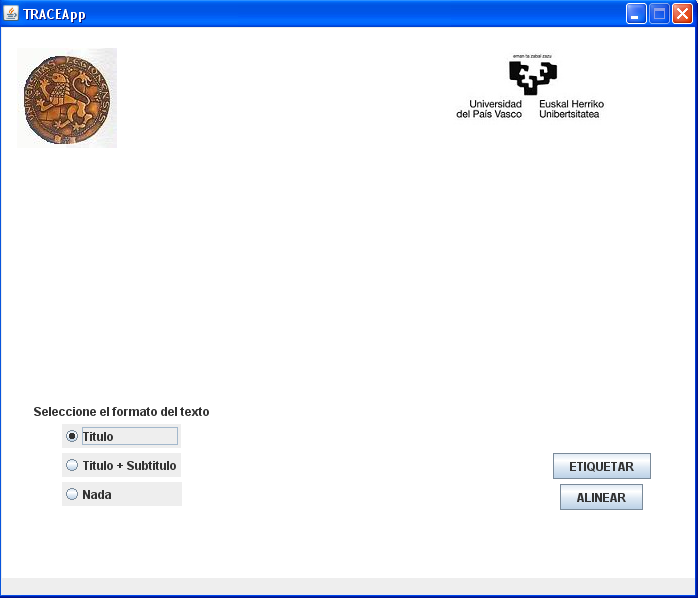
\includegraphics[width=.5\textwidth]{./figures/6-1.png}
\caption{Interface of the tagging/aligning program} \label{fig:3:1}
\end{figure}

Firstly, each text was automatically annotated in \textsc{xml} by automatically adding paragraph and sentence boundaries, to which a header containing metadata (title, author, translator, code, language, translation mode and genre) was added. Providing the texts with metadata becomes essential to subsequently exploit the corpus, as it allows the definition of subcorpora in the queries, i.e. to only search in assumed direct translations, for example, or only in indirect translations. \figrf{fig:3:2} is an example of \textsc{xml} annotation.

\begin{figure}
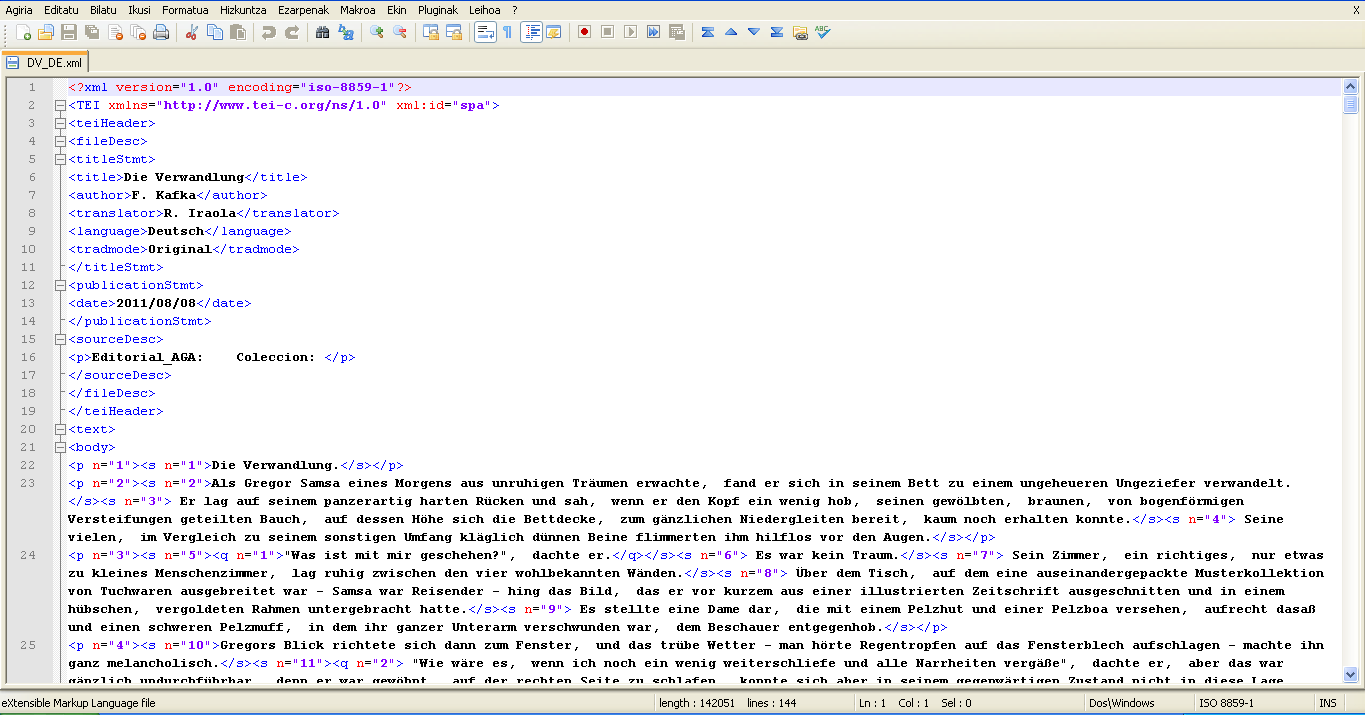
\includegraphics[width=1.0\textwidth]{./figures/6-2.png}
\caption{\textsc{xml} annotation of sample text} \label{fig:3:2}
\end{figure}

Once the texts are annotated, our software tool performs the automatic alignment of the source text and of up to two target texts.\footnote{The latest version of the program, TRACE-aligner 3.0, can align multiple texts.}  That is, the program will automatically align the tagged \textsc{xml} files at the sentence level. The result can be seen in \figref{fig:3:3}. Given that in any translation process one sentence does not necessarily correspond to another, a third step was necessary: the final fine-tuning using manual alignment.

\begin{figure}[htp] 
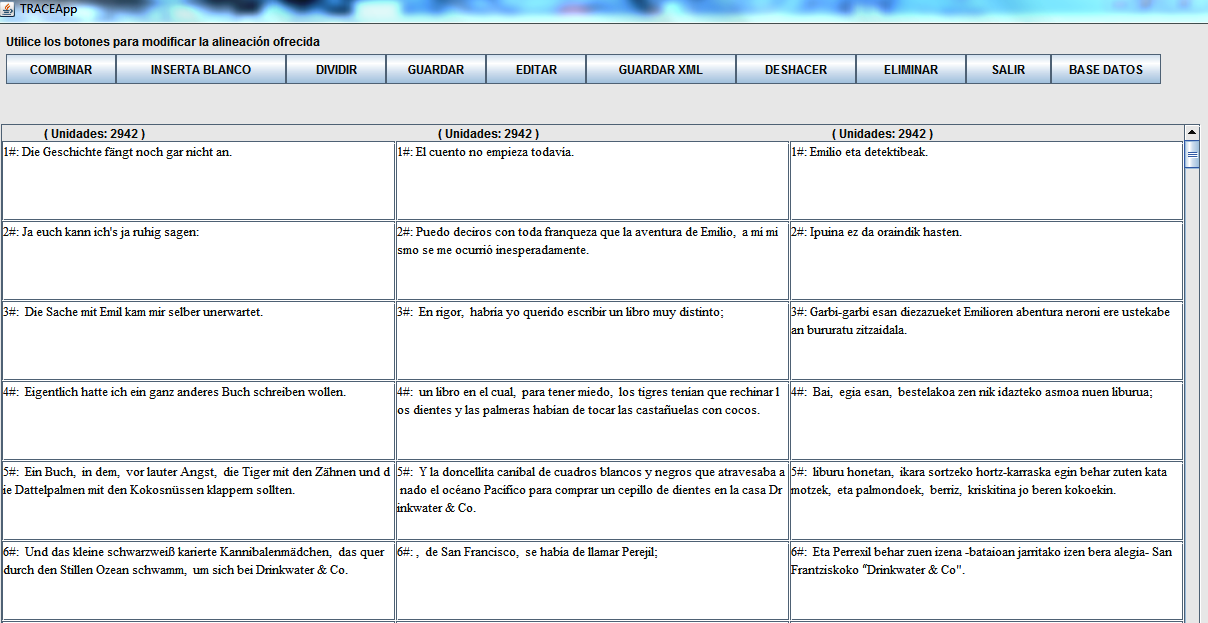
\includegraphics[width=1.0\textwidth]{./figures/6-3.png}
\caption{Sample output of automatic alignment} \label{fig:3:3}
\end{figure}

In order to manually edit the results of automatic alignment, we added different editing options to the program, such as “combine", “add cell", “edit" or “split", to make the tool as versatile and as easy to use as possible. The aim during manual alignment editing was to reflect the structure of the original text. This process is absolutely necessary, as different translations of a source text could vary significantly in terms of syntax and sentential structure, and the results displayed by the search engine depend on the alignment modifications made at this stage in accordance with the source text. The outcome of this process is shown in \figref{fig:3:4}.

\begin{figure}
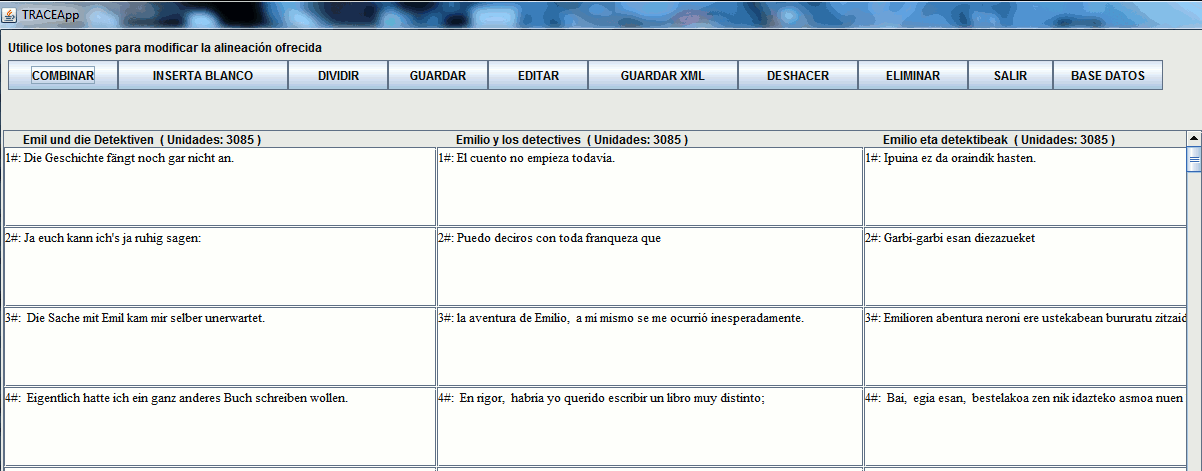
\includegraphics[width=1.0\textwidth]{./figures/6-4.png}
\caption{Sample of output after manual alignment editing} \label{fig:3:4}
\end{figure}

\subsubsection{Making queries in the database} 
The tagging/aligning program allows the user to upload the aligned texts into a MySQL database management system (we used the program Xampp for that purpose). \figref{fig:3:5} shows an image of the database management interface.

\begin{figure} 
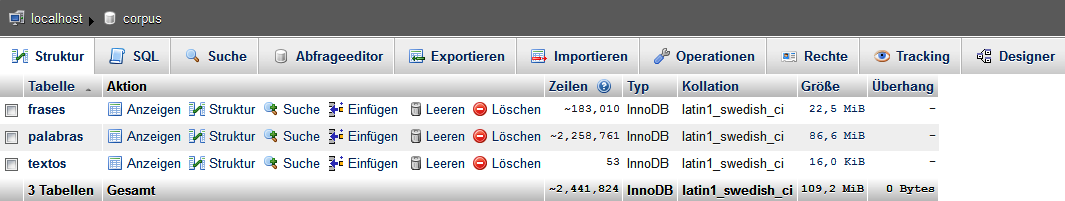
\includegraphics[width=1.0\textwidth]{./figures/6-5.png}
\caption{Image of the MySQL database, where the aligned texts are uploaded} \label{fig:3:5}
\end{figure}

Once the aligned texts are uploaded into the database, it is possible to carry out searches using a specifically developed search engine. The inclusion of metadata associated with each text makes it possible to define specific searches: by defining a given language, searches on the source- or the target-text are possible, or the search can be limited to a specific author or translator. As such, different ad hoc subcorpora can be defined with the search criteria. The search engine interface is shown in \figref{fig:3:6}.


\begin{figure} 
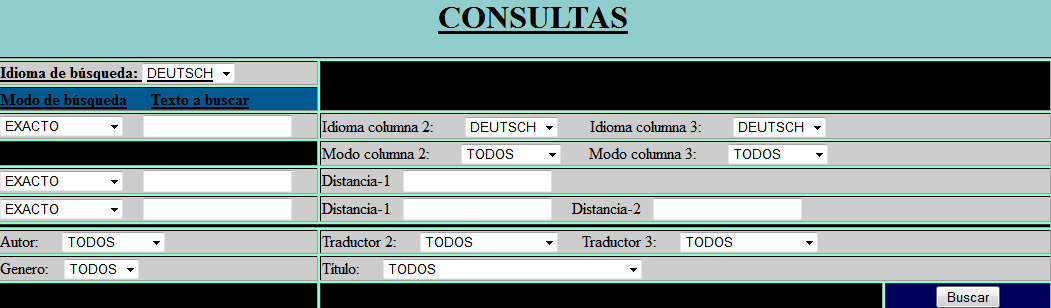
\includegraphics[width=0.9\textwidth]{./figures/6-6.png}
\caption{The search engine linked to the database} \label{fig:3:6}
\end{figure}

\figref{fig:3:7} shows the results of a search as displayed by the search engine. In this example, the search criteria are German sentences containing the words “Nagel” and “Kopf”. The first column contains the code for the aligned texts, the second column the original German text, the third, when applicable, the mediating Spanish texts and the last column the target texts in Basque. Another important feature is that the results are always contextualised: in addition to the sentence containing the words searched for, the preceding and the following sentences are also displayed.

\begin{figure}
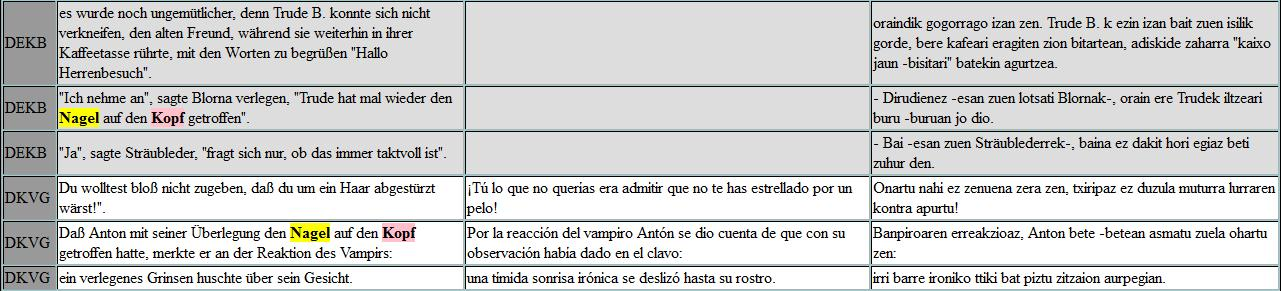
\includegraphics[width=0.9\textwidth]{./figures/6-7.jpg} 
\caption{Example of the results of a search in the corpus} \label{fig:3:7}
\end{figure}

\section{Preliminary results}
As a result of the process described above, we have created a digital, multilingual and parallel corpus, which is relatively small (over 5 million words) and topic-specific. It may not be a large corpus, but given that it was created according to the criteria which suited our research needs (see \sectref{sec:3:2}), it does provide a representative sample of the textual reality we observed. Although the main aim of this article is to describe the process of creating the corpus and the corpus itself\footnote{We continue to develop TRACE-Aligner and we hope to incorporate text analysis features in the near future (word count, word lists, word frequencies, automatic extraction of collocations and so on).}, this section presents two examples we have extracted from the corpus and which served as data for our research projects to illustrate how the corpus can be exploited.

A first example comes from \citeauthor{Zubillaga2013}'s \citeyear{Zubillaga2013} research on insults in German texts translated into Basque, using the AleuskaHGL subcorpora. In order to search for the most common insults in German, Scheffler's list (2000) was used as a reference. The insults in the list were queried one by one in the search engine and then the results were systematically analysed, paying special attention to cases of standardisation and interference. The following is an example of an indirect translation, that is, the Basque translator never looked at the German, but solely used the Spanish version. The search engine displays the three aligned texts so that we can observe the history of the entire translation process. In this case, the translation was carried out in two separate steps: the work was first translated from German into Spanish, and the Basque translation was conducted three years later, taking the mediating Spanish text as its actual source text. This example, along with various others, was classified as a case of standardisation of an insult.


\begin{table}
     \centering
     \begin{tabularx}{\textwidth}{XXX}
     \lsptoprule
OT 			& MT     & \textsc{tt}  \\ 
\midrule
Mein Kind soll keine \textbf{hochnäsige Gans} werden (Kästner 1931).   & Mi hija no debe convertirse en un \textbf{ganso orgulloso} (Kästner 1987).   & Nire alaba ezin da izan \textbf{antzara harroa} (Kästner 1989). \\ 
{[}My child won't be an arrogant goose. (meaning: \textbf{arrogant}){]} & {[}My daughter won't become an arrogant goose. (meaning: \textbf{an arrogant fool}){]}  & {[}My daughter cannot be an arrogant goose (meaning: \textbf{an arrogant goose}, meaning literally the animal){]}  \\

\lspbottomrule
\end{tabularx}

 \caption{Example of indirect translation}
     \label{3.3}
     % Verweis im Text mittels \REF{tbl:beispieltabelle}
\end{table}


\textit{A hochnäsige Gans} is somebody who is arrogant or stuck-up. The Spanish version uses the equivalent \textit{ganso orgulloso}, which is a literal translation. \textit{Ganso} is an insult in Spanish, but actually has the meaning of somebody foolish, not arrogant, although that is compensated with \textit{orgulloso}, which means arrogant. The Basque version departs from the Spanish version and also gives the literal translation of the Spanish version, i.e. the dictionary equivalent: \textit{antzara harroa}, but \textit{antzara} [goose/Gans] has no insulting connotation in Basque, it just has the literal meaning for that type of animal. The final Basque target text is, therefore, standardised, since we understand that the toning down of the offensive language reveals the standardisation of the same. In this example, the insult is completely lost compared to the mediating Spanish text, and we were able to observe that the meaning of the insult in the Spanish version is somewhat modified compared to the original German text. In summary, the literal translation from German into Spanish modifies the meaning, as \textit{Gans} and \textit{ganso} have different connotations in German and Spanish; and the literal translation of the Spanish version into Basque normalises the special meaning attached to \textit{ganso}, since \textit{antzara} has no association with foolish behaviour as is the case in Spanish, nor does it have any relation to arrogance as in German.

Example 2 arose from the AleuskaPhraseo subcorpora, as \citet{Sanz2014} was conducting her analysis on German Phraseology translated into Basque. The example is from an assumed direct translation; that is, the text had supposedly been translated directly from the German original version, and so we digitised and aligned just the German and the Basque versions\footnote{Until now, Spanish translations were included in the corpus only when the original texts had been translated through a mediating text. During our research, we realised that it would be very interesting to have the opportunity to consult the Spanish translation in all cases, also when translations were presumably made from the German original, in order to check if there is any relationship between the Spanish and Basque texts. Therefore, the systematic inclusion of the Spanish translations in the corpus is something we intend to do in the future.}. This is an example of what we called diglossic interference or interference of the dominant language (Spanish, in this case), as described above.

\begin{table}
     \centering
     \begin{tabularx}{\textwidth}{XX}
     \lsptoprule
German original    & Spanish bridge version  \\ 
\midrule
Kann jedem mal passieren, daß \textbf{ihm die Hand ausrutscht}, wenn er in Rasche ist".	(Döblin 1929).   &  Edonori gertatzen zaiok, amorrazita dagoenean \textbf{eskuak alde egitea}". (Döblin 2000).  \\ 
{[}It can happen to anyone that, when he/she gets angry, his/her hand slips (meaning: someone gives another person a slap in the face){]}  & {[}It can happen to anyone that, when he/she gets angry, his/her hand runs away{]}  \\

\lspbottomrule
\end{tabularx}

 \caption{Example of a diglossic interference}
     \label{3.4}
     % Verweis im Text mittels \REF{tbl:beispieltabelle}
\end{table}     
   
As we can see in the German version, the author uses the German idiom \textit{jmdm rutscht die Hand aus} which - according to Duden 11, a German monolingual dictionary specialised in German idioms and proverbs– has the following meaning “jmd. gibt jmdm. eine Ohrfeige". In other words, the actual meaning of the PU is to give someone a slap in the face, and word for word it can be translated as "someone's hand slips". In the Basque translation, we do not find a PU. We were not able to find the expression used in the Basque version in any dictionary and when we searched for this word combination (“eskuak alde egin") in the large corpora mentioned in \sectref{sec:3:1} (ETC corpus), we found no occurrences. We believe that the translator has made a literal translation of a Spanish PU, which is “escapársele a alguien la mano"\footnote{According to María Moliner, a well-known Spanish monolingual dictionary, it means “no poder contenerse de hacer cierta cosa" or not to be able to stop oneself from doing something.}, because the Basque version is a 'word for word' translation. We cannot explain the process of this translation without taking into account that the translator of this text is a diglossic translator, living in a diglossic community, using indirect tools to translate (i.e. German-Spanish dictionaries first, and Spanish-Basque dictionaries afterwards).\footnote{No German-Basque dictionaries existed at the time of the translation in question.} For these reasons, we consider this to be a case of diglossic interference.

The two cases presented above have shown how we have used the search tool in order to retrieve data from the corpus on the one hand and, on the other, how translation behaviour has been analysed in the framework of our research projects. Example 1\todo{Usage of \emph{Example} and \textbackslash \{table\} in this chapter needs to be checked}, in the context of an indirect translation process, shows a case of toning down, which we link with the law of standardisation. Example 2 represents a case of interference which, however, does not stem from the German source text but rather from the translator diglossic competence. In this and other cases, although the translation was nominally direct from German, the Basque target texts contained interferences from another language, Spanish in our case.

\section{Conclusions}

The aim of this article was to explain and present the steps we undertook to build up our corpora and to report initial results. Thanks to the teamwork with our computer technician, we were able to create a user-friendly program and with its help we can now build up our own digitalised, aligned and searchable multilingual corpora.

On the technical side, we are developing TRACE-Aligner 3.0. The updated and improved version can now align more than 3 texts and the database production is much simpler. We will next integrate some text analysis features, starting with those present in model tools like AntConc\footnote{\url{http://www.laurenceanthony.net/antconc_index.html}} and WordSmith Tools. We are also working on the integration of all three existing subcorpora into one general German to Basque parallel corpus consisting of over 5 million words, which will be soon locally available for internal use among researchers of our faculty. The publication of the entire corpus or parts thereof is under consideration, but this move is hindered by copyright issues.

In the matter of use and exploitation, our work is at an early stage; however, we were able to identify both standardisation and interference at work in a context, where the development of a standard form of Basque is an additional factor. Our initial results (for example, regarding different types of interference) now need to be checked with further studies. On the other hand, the process of creating our corpus is a long-term investment which can have many different applications in the future. It can be the departing point for further empirical and systematic research on German to Basque translations and may also play a role in translation didactics, lexicography, contrastive linguistics and other related areas. Our corpus could also serve as a model for similar work with translations from other source languages into Basque and, in the process, could help broaden the picture to the larger field of translations into Basque.


\section*{Acknowledgements}

We would like to thank our computer technician, Iñaki Albisua, who has developed TRACE-Aligner 2.0 and TRACE-Aligner 3.0.

\printbibliography[heading=subbibliography,notkeyword=this]

\end{document}